\documentclass[11pt]{article}

% ---------- encoding & fonts ----------
\usepackage[utf8]{inputenc}
\usepackage[protrusion=true,expansion=false]{microtype}

% ---------- layout ----------
\usepackage[a4paper,margin=1in]{geometry}
\usepackage{titlesec}
\usepackage{enumitem}
\setlist{leftmargin=1.4em,itemsep=2pt,topsep=3pt}

% ---------- color ----------
\usepackage{xcolor}
\definecolor{indigo}{HTML}{4130C9}
\definecolor{indigoB}{HTML}{5B47F5}
\definecolor{amber}{HTML}{9A6410}
\definecolor{amberB}{HTML}{D9971C}
\definecolor{ink}{HTML}{161A22}
\definecolor{muted}{HTML}{6B7280}
\definecolor{codebg}{HTML}{F4F5F8}
\definecolor{rulegray}{HTML}{D1D6DE}
\definecolor{ok}{HTML}{2E7D57}

% ---------- tables ----------
\usepackage{booktabs}
\usepackage{tabularx}
\usepackage{array}
\renewcommand{\arraystretch}{1.22}\setlength{\tabcolsep}{5pt}\emergencystretch=3em
\newcolumntype{Y}{>{\raggedright\arraybackslash}X}

% ---------- code ----------
\usepackage{listings}
\usepackage[obeyspaces]{url}
\urlstyle{tt}
\lstdefinestyle{lr}{
  basicstyle=\ttfamily\footnotesize,
  backgroundcolor=\color{codebg},
  frame=single,framerule=0pt,rulecolor=\color{rulegray},
  framesep=7pt,xleftmargin=7pt,xrightmargin=7pt,aboveskip=10pt,belowskip=6pt,
  breaklines=true,breakatwhitespace=false,
  commentstyle=\color{muted}\itshape,
  keywordstyle=\color{indigo}\bfseries,
  stringstyle=\color{amber},
  showstringspaces=false,
  morecomment=[l]{\#},
  morestring=[b]",morestring=[b]',
  morekeywords={POST,GET,from,import,Bearer},
  columns=fullflexible,keepspaces=true,
}
\lstset{style=lr}


% ---------- graphics ----------
\usepackage{tikz}
\usetikzlibrary{positioning,arrows.meta,fit,backgrounds,calc}
\usepackage{graphicx}

% ---------- section styling ----------
\titleformat{\section}{\Large\sffamily\bfseries\color{ink}}{\color{indigo}\thesection\hspace{0.5em}}{0em}{}
\titleformat{\subsection}{\large\sffamily\bfseries\color{ink}}{\color{indigo}\thesubsection\hspace{0.5em}}{0em}{}
\titlespacing*{\section}{0pt}{16pt}{6pt}
\titlespacing*{\subsection}{0pt}{12pt}{4pt}
\renewcommand{\thesubsection}{\arabic{section}.\arabic{subsection}}

% ---------- remark environment (matches EMS guide run-in style) ----------
\newenvironment{remark}
  {\par\medskip\noindent\small\itshape\textbf{\upshape Remark.}\hspace{0.4em}\ignorespaces}
  {\par\medskip}

% ---------- hyperref (load late) ----------
\usepackage[colorlinks=true,linkcolor=indigo,urlcolor=indigo,citecolor=indigo]{hyperref}
\makeatletter
\g@addto@macro\UrlBreaks{\do\_\do\/\do\.\do\:\do\,\do\;\do\-\do\(\do\)\do\{\do\}\do\*\do\=\do\'\do\"%
\do\A\do\B\do\C\do\D\do\E\do\F\do\G\do\H\do\I\do\J\do\K\do\L\do\M\do\N\do\O\do\P\do\Q\do\R\do\S\do\T\do\U\do\V\do\W\do\X\do\Y\do\Z}
\makeatother
\DeclareUrlCommand\co{\urlstyle{tt}}


\title{\vspace{-1.2cm}\sffamily\bfseries The Light Rider Cloud Platform:\\[2pt]
\large Self-Serve Quantum Compute and Attested Entropy}
\author{\normalsize Light Rider Inc. --- Engineering}
\date{\normalsize August 7, 2026 \quad\textbullet\quad Internal (Dev / Ops)}

\begin{document}
\maketitle
\vspace{-0.7cm}
\begin{center}\small\itshape
Companion to ``The Light Rider Platform: Attested Multi-Source Entropy as a Service'' (2026-07-14).\\
Verified against the \co{cloud_platform_nextjs} source tree on 2026-08-07.
\end{center}

\noindent\textbf{Abstract.}\enspace
The cloud platform is the customer-facing surface of Light Rider: a Next.js~16 application on Vercel, served from
\co{platform.lightriderinc.com}, that lets a user run circuits on IQM quantum processors and draw attested entropy
\emph{without holding an IQM credential or operating the entropy backend}. It is a control-and-UI layer with a thin
server API. Identity and roles come from Logto; the platform keeps Stripe-facing billing state --- customers,
subscriptions, a prepaid credit ledger, API keys, and a record of submitted jobs --- while the lr\,/\,EMS backend calls
back to check balances before running work. Every capability is served through server route handlers that attach the
right upstream credential and call one of two services: the EMS entropy egress (the companion guide's subject) and
iqm-proxy for circuit execution. The platform's defining job is to present those services as a metered, credentialed
product while keeping their credentials server-side. This guide defines the platform's vocabulary, its architecture and
request flows, its auth\,/\,billing\,/\,credential subsystems, how it consumes EMS, its deploy and operations model, and
the work in progress.

\medskip
\noindent\fcolorbox{rulegray}{codebg}{\begin{minipage}{0.97\linewidth}\small
\textbf{Provenance.}\enspace Endpoints, environment-variable names, backend ids, pricing, and the entropy
source\,$\rightarrow$\,policy map below are read from the code (routes, clients, \co{prisma/schema.prisma},
\co{.env.example}, \co{logto.ts}, the backend catalog, the Colab notebooks), not inferred. Items marked
\emph{[open]} are repo-flagged TODOs or operational details to settle, not gaps in this write-up.
\end{minipage}}

\medskip
{\small\tableofcontents}
\bigskip

% ============================================================
\section{Problem statement}
Two upstream services do the real work, and both are awkward to consume directly. Running circuits on IQM means holding
an IQM service token and building an IAM around it; drawing entropy from EMS means operating the backend, passing a
privileged key, and verifying signed receipts. Neither is something a customer should have to do, and neither credential
should ever reach a browser.

The platform resolves this by being a single hosted origin. A user signs in with Google or GitHub, receives an API key,
and then runs circuits and draws entropy through \textbf{one domain}. The platform holds the privileged upstream
credentials --- the IQM service token (behind iqm-proxy) and the EMS key --- \textbf{server-side only}, and re-exposes
IQM's backends and EMS's pools and policies as product features. Compute is charged against a prepaid credit ledger;
entropy is entitlement-gated at EMS.

\begin{remark}
\textbf{\upshape Where state lives.} The Prisma schema is deliberately scoped to \emph{Stripe-facing} state only (who the
customer is in Stripe, what they are subscribed to, a credit ledger). It does not model quantum jobs, entropy pools, or
usage enforcement --- that lives in the lr\,/\,EMS backend, which is expected to call back into this app (or read a
synced replica) to check balances before running work (see \co{BILLING_INTEGRATION.md}). The platform is the commerce
and identity system of record; the backend is the compute system of record.
\end{remark}

\begin{remark}
\textbf{\upshape No second trust root.} The platform adds no cryptographic guarantee of its own. Entropy attestation
lives entirely in EMS's signed receipt, verified against the EMS public key; circuit results carry iqm-proxy's job
identity. The platform's contribution is productization --- identity, metering, keys, a coherent surface --- not a
second trust root.
\end{remark}

% ============================================================
\section{Preliminaries}
This section defines the platform's vocabulary. It assumes the entropy concepts from the EMS guide (min-entropy,
extractors, receipts, pools, policies) and adds the platform's own terms.

\subsection{Runtime}
\textbf{Next.js App Router} (v16 --- a major with breaking changes; \co{AGENTS.md} tells contributors to read the
bundled docs before writing code). React components render the UI; \emph{route handlers} under \co{src/app/api/} are the
server API and the only place secrets exist. \textbf{Vercel} hosts it; a push to \co{main} triggers a production build
(\S\ref{sec:deploy}).

\subsection{Identity, billing, storage}
\textbf{Logto} (\co{@logto/next}) owns sign-in, Google\,/\,GitHub OAuth, sessions, and the \textbf{Basic}\,/\,\textbf{Pro}
roles. \textbf{Stripe} owns payments. The platform keeps a \textbf{credit ledger} (append-only, signed cents) for prepaid
\textbf{Quantum Compute credits}, and separately reports \textbf{EaaS API usage} to a Stripe Billing Meter.
\textbf{Prisma} is the ORM over \textbf{Postgres} (\co{DATABASE_URL} + \co{DIRECT_URL}; SQLite for local dev).
\textbf{Supabase} appears only as object storage for user avatars.

\subsection{Upstream services}
\textbf{EMS} egress is reached at \co{EMS_BASE_URL}; the platform authenticates with a \textbf{Bearer} key that EMS
resolves against tier entitlements. \textbf{iqm-proxy} is reached at \co{QUANTUM_PROXY_URL} --- confirmed at
\co{http://93.127.215.63} (iqm-proxy fronted by nginx on the bare IP, port~80). \textbf{device\_instance routing} is a
body field on each submission naming the QPU alias (\co{garnet}, \co{garnet:mock}, \dots) that iqm-proxy's device
registry expects. A \textbf{mock backend} is a \co{:mock} alias that runs on iqm-proxy's statevector simulator, free and
unlimited.

\begin{remark}
Several credentials share the \co{lr_} prefix and the word ``key'' --- the user's platform API key, the quantum-proxy
service key, and the legacy entropy token are all distinct. They are enumerated definitively in
\S\ref{sec:keys}; read that before wiring anything.
\end{remark}

% ============================================================
\section{Architecture}
One origin, strict client\,/\,server split. The React UI runs in the browser; route handlers run on Vercel and are the
only place upstream credentials live. The browser never contacts EMS, iqm-proxy, Stripe's secret API, or the database
directly --- every such call is proxied through a same-origin route.

\begin{table}[h]
\centering\small
\begin{tabularx}{\linewidth}{@{}>{\raggedright\arraybackslash}p{0.19\linewidth} Y >{\raggedright\arraybackslash}p{0.30\linewidth}@{}}
\toprule
\textbf{Concern} & \textbf{Technology} & \textbf{Notes}\\
\midrule
Web app + API & Next.js 16.2.9, React 19, TypeScript, Tailwind~v4 & UI + route handlers, one deployable\\
Hosting / CI & Vercel; semantic-release on \co{main} & push $\to$ build; release bot commits \co{CHANGELOG}\\
Identity & Logto (\co{@logto/next}) & sign-in via \co{auth.lightriderinc.com}; roles Basic\,/\,Pro\\
Billing & Stripe (\co{stripe} v22): Checkout, subs, webhooks, meter & test-mode until live is signed off\\
Database / ORM & Prisma 6 over Postgres (\co{DATABASE_URL}) & SQLite for local dev; Supabase = avatars\\
Entropy backend & EMS egress via \co{EMS_BASE_URL} & Bearer entitlement; \co{/v1/entropy/*}\\
Circuit exec & iqm-proxy via \co{QUANTUM_PROXY_URL} & \co{93.127.215.63}:80; six IQM backends + mock\\
Client SDK & \co{lightrider} (PyPI) v1.3.1; Colab notebooks & talks to the platform with an \co{lr_} key\\
PQC primitives & \co{@noble/post-quantum}, \co{@noble/hashes} & Vault (ML-KEM-768) / Signer (ML-DSA-65)\\
\bottomrule
\end{tabularx}
\caption{Technology by concern (versions from \texttt{package.json}).}
\end{table}

\begin{figure}[h]
\centering
\resizebox{\linewidth}{!}{%
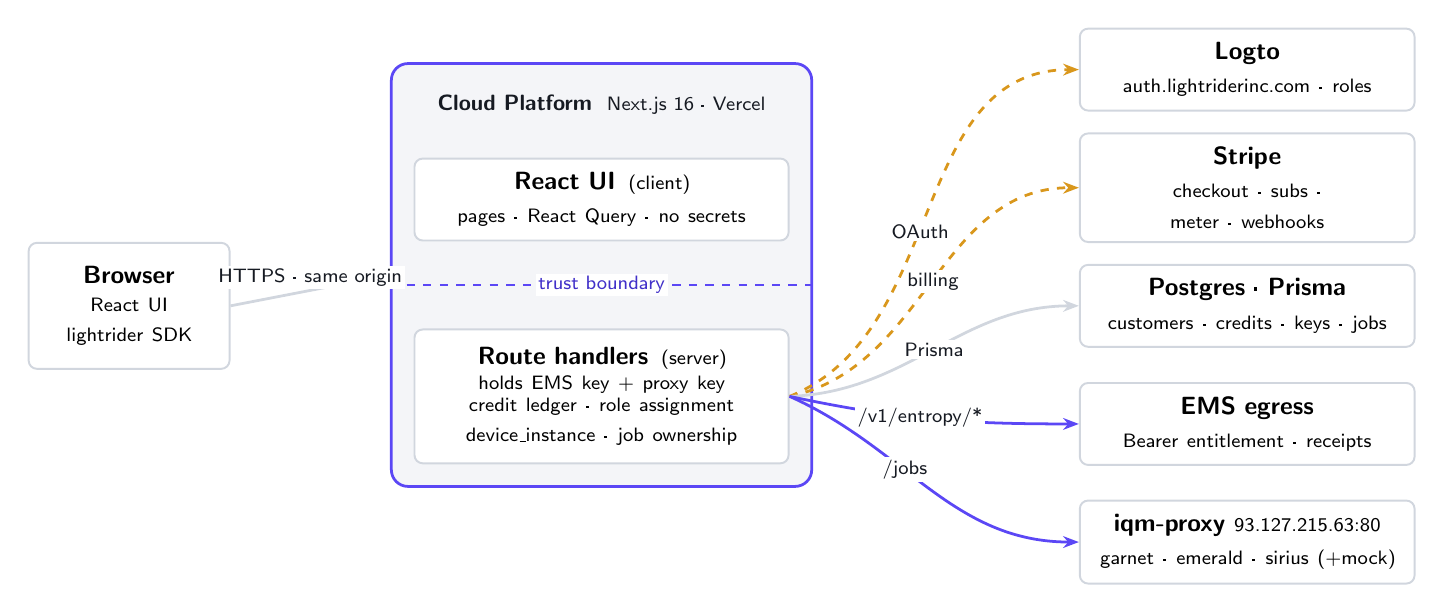
\begin{tikzpicture}[
  font=\sffamily\small,
  box/.style={draw=rulegray,rounded corners=3pt,line width=0.7pt,align=center,inner sep=5pt},
  svc/.style={box,fill=white,text width=3.9cm,minimum height=1.0cm},
  data/.style={-{Stealth[length=2mm]},indigoB,line width=1pt},
  ctrl/.style={-{Stealth[length=2mm]},amberB,line width=1pt,dashed},
  neu/.style={-{Stealth[length=2mm]},rulegray,line width=1pt},
  lbl/.style={font=\sffamily\scriptsize,fill=white,inner sep=1pt,text=ink},
]
% browser
\node[box,fill=white,text width=2.2cm,minimum height=1.6cm] (br) at (-0.6,0) {\textbf{Browser}\\[2pt]\scriptsize React UI\\\scriptsize lightrider SDK};

% platform sub-boxes
\node[box,fill=white,text width=4.4cm,minimum height=1.0cm] (ui) at (5.4,1.35) {\textbf{React UI} \,\scriptsize(client)\\[1pt]\scriptsize pages · React Query · no secrets};
\node[box,fill=white,text width=4.4cm,minimum height=1.7cm] (srv) at (5.4,-1.15) {\textbf{Route handlers} \,\scriptsize(server)\\[1pt]\scriptsize holds EMS key + proxy key\\\scriptsize credit ledger · role assignment\\\scriptsize device\_instance · job ownership};
\node[font=\sffamily\bfseries\footnotesize,text=ink] (ptitle) at (5.4,2.55) {Cloud Platform \;\scriptsize\mdseries Next.js 16 · Vercel};
% platform frame on background
\begin{scope}[on background layer]
\node[draw=indigoB,line width=1pt,rounded corners=6pt,fill=codebg,fit=(ui)(srv)(ptitle),inner sep=8pt] (plat) {};
\end{scope}
% trust boundary
\coordinate (mid) at ($(ui.south)!0.5!(srv.north)$);
\draw[dashed,indigoB,line width=0.6pt] (plat.west|-mid) -- (plat.east|-mid);
\node[lbl,text=indigo] at (mid) {trust boundary};

% services
\node[svc] (logto)  at (13.6,3.0)  {\textbf{Logto}\\[1pt]\scriptsize auth.lightriderinc.com · roles};
\node[svc] (stripe) at (13.6,1.5)  {\textbf{Stripe}\\[1pt]\scriptsize checkout · subs · meter · webhooks};
\node[svc] (pg)     at (13.6,0.0)  {\textbf{Postgres · Prisma}\\[1pt]\scriptsize customers · credits · keys · jobs};
\node[svc] (ems)    at (13.6,-1.5) {\textbf{EMS egress}\\[1pt]\scriptsize Bearer entitlement · receipts};
\node[svc] (iqm)    at (13.6,-3.0) {\textbf{iqm-proxy} \scriptsize 93.127.215.63:80\\[1pt]\scriptsize garnet · emerald · sirius (+mock)};

% edges browser<->platform
\draw[neu] (br.east) -- node[lbl,above]{HTTPS · same origin} (plat.west);
% edges server->services (labels placed mid-path, white fill)
\draw[ctrl] (srv.east) to[out=22,in=180]  node[lbl,pos=0.45]{OAuth} (logto.west);
\draw[ctrl] (srv.east) to[out=12,in=180]  node[lbl,pos=0.5]{billing} (stripe.west);
\draw[neu]  (srv.east) to[out=2,in=180]   node[lbl,pos=0.5]{Prisma} (pg.west);
\draw[data] (srv.east) to[out=-12,in=180] node[lbl,pos=0.45]{/v1/entropy/*} (ems.west);
\draw[data] (srv.east) to[out=-24,in=180] node[lbl,pos=0.4]{/jobs} (iqm.west);
\end{tikzpicture}}
\caption{Platform overview. The browser talks to exactly one origin. Upstream credentials (the IQM token behind
iqm-proxy, the EMS key) live only inside server route handlers and never cross the trust boundary. Indigo paths carry
data (entropy bytes, circuit jobs); amber paths carry control (identity, billing). Not shown: per-vendor pass-through
proxies (\texttt{/api/iqm}, \texttt{ibm}, \texttt{rigetti}, \texttt{nist}, \texttt{curby}, \texttt{drand}, \texttt{anu}) the catalog and legacy
entropy path use.}
\end{figure}

% ============================================================
\section{Data flow}
Three request families cover almost everything. Each begins in the UI or SDK and terminates in a server route handler
that attaches the right credential and calls upstream.

\subsection{Draw entropy}
The main path is the EMS-backed console (\co{/entropy}). A separate legacy path serves the Quantum Vault ``try a
source'' tab.
\begin{enumerate}
\item \textbf{UI request.} \co{requestEntropy()} (\co{src/lib/entropy/generate.ts}) maps the chosen source card to an EMS
policy and calls \co{POST /api/ems/entropy} with \co{{mode:"single",policy,bytes}}. A multi-source draw sends
\co{{mode:"multi",method,sourceIds,bytes}}.
\item \textbf{Server route.} \co{/api/ems/entropy} requires a signed-in Logto user (401 otherwise) and requires
\co{EMS_BASE_URL} (500 otherwise).
\item \textbf{Call EMS.} It forwards to \co{EMS_BASE_URL} + \co{/v1/entropy/request} (single) or \co{/v1/entropy/multi}
(multi), sending \co{Authorization: Bearer $EMS_API_KEY} and an (inert) \co{x-ems-api-key}.
\item \textbf{EMS responds.} \co{bytes_hex} plus the full signed receipt (sources, quality, credited min-entropy,
\co{audit_event_id}, signature). The route returns EMS's body verbatim.
\item \textbf{Render + record.} The client keys a history entry on \co{receipt.request_id} and derives \co{createdAt}
from \co{receipt.timestamp_unix_ns}.
\end{enumerate}

\begin{lstlisting}[caption={server route to EMS egress (from src/app/api/ems/entropy/route.ts)},captionpos=b]
POST $EMS_BASE_URL/v1/entropy/request        # or /v1/entropy/multi
Authorization: Bearer $EMS_API_KEY           # the real auth (entitlement-resolved)
x-ems-api-key: $EMS_API_KEY                  # inert until EMS grows a route that reads it
{ "bytes": 32, "policy": "quantum_verified",
  "application_id": "", "zone_id": "", "client_nonce": "" }
\end{lstlisting}

\begin{remark}
\textbf{\upshape Entitlement, not role.} EMS resolves the Bearer key against tier entitlements
(\co{ems-egress/src/entitlement.rs}). An \emph{anonymous} or under-entitled key is silently downgraded to the Free
grant, which can only draw \co{pool_fastest} and never gets \co{multi_source}. The product intent is ``no
role\,/\,subscription gate on source selection,'' so \co{EMS_API_KEY} must be a fully-entitled key or signed-in users
quietly lose sources (\S\ref{sec:wip}).
\end{remark}

\noindent\textbf{Legacy path --- \co{GET /api/entropy?source=\&bytes=}.}\enspace Used by Quantum Vault's ``My Keys'' tab
to try a source without EMS. \co{nist-beacon} hits NIST's real Randomness Beacon~2.0; otherwise, if \co{LR_TOKEN} is set,
it runs an \co{h}-gate job on the LR quantum API and HKDF-derives bytes from \co{jobId + counts}; failing both, it
returns \co{randomBytes} honestly labeled \co{X-Entropy-Source: csprng-fallback}. This is the one place a CSPRNG fallback
still exists --- the EMS console path never falls back.

\subsection{Run a circuit}
Circuit submission proxies to iqm-proxy with a shared service key; the customer never sees an IQM token.
\begin{enumerate}
\item \textbf{Submit.} UI or SDK sends \co{{backend,circuit,shots}} to \co{POST /api/lr/quantum/submit}, authenticated by
a Logto session \emph{or} an \co{Authorization: Bearer lr_...} key (\co{resolveCustomerFromRequest}). First-ever request
lazily creates the Customer and grants the free signup credit.
\item \textbf{Gate on credits.} Cost = \co{ceil(shots * costPerShotCents)}. Real QPUs require having purchased credits at
least once ($\to$ \co{402 purchase_required}); then an insufficient balance ($\to$ \co{402 insufficient_credits}). Mock
backends cost 0, so both checks no-op.
\item \textbf{Route + call.} The handler resolves the backend to its \co{deviceInstance} and calls \co{QUANTUM_PROXY_URL}
+ \co{/jobs} with \co{Authorization: Bearer $QUANTUM_PROXY_SERVICE_KEY} and body \co{{circuit,shots,device_instance}}.
\item \textbf{Record atomically.} On success it writes a \co{QuantumJobSubmission} row and, if billable, decrements
\co{creditsBalanceCents} + appends a negative \co{CreditLedgerEntry} --- all in one \co{db.$transaction}.
\item \textbf{List + poll.} \co{GET /api/lr/quantum/jobs} returns the caller's own rows (cached status); the client
re-polls live status per non-terminal job, and \co{finishedAt} is backfilled from iqm-proxy opportunistically.
\end{enumerate}

\begin{lstlisting}[language=Python,caption={what a customer runs (from docs/notebooks/quantum-quickstart-iqm-garnet.ipynb)},captionpos=b]
# %pip install -q lightrider==1.3.1 requests
from lightrider import Circuit, get_backend

local = get_backend("statevector")           # free local sim, no key needed

base_url = "https://platform.lightriderinc.com"
session.headers["Authorization"] = f"Bearer {api_key}"   # lr_ key from /settings/keys

session.post(f"{base_url}/api/lr/quantum/submit",
    json={"backend": "iqm-garnet-mock", "circuit": circuit, "shots": 1000})
# poll {base_url}/api/lr/quantum/jobs/{id}  then  /result
\end{lstlisting}

\noindent\textbf{Two submission generations.}\enspace \co{/api/lr/quantum/submit} (current) takes a full circuit object
\co{{num_qubits,instructions:[{name,qubits,clbits?}]}}. The older \co{/api/lr/jobs} took \co{{gate,shots}} shorthand and
is still used by the legacy entropy path and \co{src/lib/lr/client.ts}. Presets \co{h}\,/\,\co{bell} live in
\co{src/lib/quantum/client.ts}.

\subsection{Authenticate \& meter}
Sign-in, role assignment, and metering --- the control plane over the two data flows.
\begin{enumerate}
\item \textbf{Sign in.} Logto (Google\,/\,GitHub via Light Rider's own OAuth apps) at \co{auth.lightriderinc.com}. New
users are Basic.
\item \textbf{Subscribe.} Stripe Checkout for the Pro plan (\$99/mo) or an API plan; a validation-only price
(\co{STRIPE_PRICE_VALIDATION_TEST}) exists to exercise the whole pipeline end to end.
\item \textbf{Reconcile.} The webhook receiver handles \co{checkout.session.completed} and
\co{customer.subscription.{created,updated,deleted}}, credits the ledger, and assigns the Logto Pro role
(\co{LOGTO_PRO_ROLE_ID}).
\item \textbf{Guard idempotency.} Every processed event id is written to \co{ProcessedStripeEvent}, and ledger grants
carry a unique \co{stripeEventId}.
\item \textbf{Meter.} Compute debits the ledger per job at submit; EaaS API overage is reported to a Stripe Billing Meter
by the backend gateway (\S\ref{sec:billing}).
\end{enumerate}

\begin{remark}
Money state is authoritative in Stripe; the ledger and cached \co{creditsBalanceCents} are the platform's idempotent
projection of it. Never let the client assert a balance.
\end{remark}

% ============================================================
\section{Authentication \& identity}\label{sec:auth}
Identity is delegated to \textbf{Logto}. Sign-in uses \textbf{Google and GitHub OAuth} on Light Rider's own apps. Config
lives in \co{src/app/logto.ts}: the sign-in endpoint (\co{auth.lightriderinc.com}) and \co{appId} are hardcoded there;
\co{LOGTO_APP_SECRET}, \co{LOGTO_COOKIE_SECRET}, and the M2M credentials come from env. Two roles exist ---
\textbf{Basic} (default) and \textbf{Pro} --- assigned from Stripe subscription state.

\medskip
\noindent\textbf{Two Logto footguns, both real in \co{logto.ts}.}
\begin{enumerate}
\item \textbf{\co{baseUrl} falls back to localhost.} It is \co{process.env.NEXT_PUBLIC_BASE_URL || 'http://localhost:3000'}.
If \co{NEXT_PUBLIC_BASE_URL} is not set for the deployed environment, OAuth callbacks resolve to localhost and sign-in
breaks. Set it everywhere (preview and production).
\item \textbf{Management API cannot use the custom domain.} The Management API token endpoint and calls must go through
the tenant's default \co{*.logto.app} domain (\co{managementEndpoint} is pinned to it), even though sign-in uses the
custom domain. Do not merge the two into one host.
\end{enumerate}

% ============================================================
\section{Billing \& credits}\label{sec:billing}
Billing runs on \textbf{Stripe} and splits into three mechanisms. The Prisma schema models only the Stripe-facing side.

\begin{table}[h]
\centering\small
\begin{tabularx}{\linewidth}{@{}>{\raggedright\arraybackslash}p{0.22\linewidth} Y >{\raggedright\arraybackslash}p{0.22\linewidth}@{}}
\toprule
\textbf{Mechanism} & \textbf{How it works} & \textbf{Where}\\
\midrule
Prepaid Quantum Compute credits & Append-only \co{CreditLedgerEntry} (signed cents); cached
\co{Customer.creditsBalanceCents}. Debited per job at submit --- \co{ceil(shots * costPerShotCents)}. Free signup grant
on first submit; real QPUs require $\geq$1 purchase. & \co{/api/lr/quantum/submit}, \co{lib/billing/}\\
Subscriptions & \co{Subscription} mirrors Stripe; \co{kind} is USER\_PLAN or API\_PLAN. User Pricing = Basic (free) + Pro
(\$99/mo, \$99 credits); Starter\,/\,Developer\,/\,Professional documented but not offered; Enterprise $\to$ Contact
Sales. API Pricing = Free\,/\,Starter (\$99)\,/\,Developer (\$499)\,/\,Business, usage-metered. & webhook,
\co{lib/billing/plans.ts}\\
EaaS API usage meter & \co{reportApiUsage()} emits a Stripe Billing Meter event + records \co{ApiUsageEvent}. Designed to
be called by the entropy API gateway (backend team), not this app. & \co{lib/billing/meter.ts}\\
\bottomrule
\end{tabularx}
\caption{The three billing mechanisms.}
\end{table}

\begin{itemize}
\item \textbf{Idempotency.} \co{ProcessedStripeEvent} logs every handled event id; ledger grants carry a unique
\co{stripeEventId}.
\item \textbf{Webhook events.} \co{checkout.session.completed}, \co{customer.subscription.{created,updated,deleted}};
unknown events are recorded and ignored.
\item \textbf{Mode.} Stripe defaults to test-mode in the example config, pending live-mode sign-off from Tony\,/\,Jake.
\end{itemize}

\begin{remark}
\textbf{\upshape Pro is parked.} The V2 job path is \emph{purely credit-gated} --- there is no Pro check anywhere in
\co{/api/lr/quantum/submit}. The Pro subscription flow, \co{isProCustomer()}, and \co{resync-pro-role} all still exist
but are unreachable from submission today.
\end{remark}

% ============================================================
\section{Credentials}\label{sec:keys}
The most confusable part of the system. User-facing keys are created in \co{/settings/keys}: a key is \co{lr_live_} /
\co{lr_test_} + 24 random bytes, stored as a \textbf{SHA-256} \co{keyHash} (Prisma \co{ApiKey}) with a short
\co{keyPrefix}, and the plaintext is shown \textbf{once}. It is sent to the platform as a Bearer token and resolves to a
\co{Customer}.

\begin{table}[h]
\centering\small
\begin{tabularx}{\linewidth}{@{}>{\raggedright\arraybackslash}p{0.30\linewidth} >{\raggedright\arraybackslash}p{0.24\linewidth} Y@{}}
\toprule
\textbf{Credential} & \textbf{Direction} & \textbf{Storage / form}\\
\midrule
Platform API key & user $\to$ platform (Bearer) & Prisma \co{ApiKey}, SHA-256 hash, shown once; \co{lr_live_}/\co{lr_test_}\\
\co{EMS_API_KEY} & platform $\to$ EMS egress & env; \co{Authorization: Bearer} (+ inert \co{x-ems-api-key}). Must be fully entitled \emph{[open]}\\
\co{QUANTUM_PROXY_SERVICE_KEY} & platform $\to$ iqm-proxy (Bearer) & env; an \co{lr_} key from iqm-proxy's own \co{/users}, one shared service account\\
\co{LR_TOKEN} & platform $\to$ LR quantum API (legacy) & env; Bearer, used only by \co{GET /api/entropy}. Parallel to the proxy key \emph{[open]}\\
\co{IQM_TOKEN} · \co{RIGETTI_TOKEN} · \co{IBM_CLOUD_API_KEY} & platform $\to$ vendor APIs & env; used by the pass-through proxies \co{/api/iqm}, \co{rigetti}, \co{ibm}\\
\bottomrule
\end{tabularx}
\caption{Every credential the platform touches.}
\end{table}

\begin{remark}
Because iqm-proxy sees only the one shared \co{QUANTUM_PROXY_SERVICE_KEY}, it cannot tell customers apart ---
per-customer job ownership is enforced locally by the \co{QuantumJobSubmission} table, which is what lets \co{jobs/[id]}
and \co{/result} reject someone else's job id. The customer's \co{lr_} key and iqm-proxy's \co{lr_} keys share a prefix
but are different namespaces; follow the endpoint to know which is which.
\end{remark}

% ============================================================
\section{Quantum compute}
Six IQM backends are wired for submission (\co{src/lib/quantum/backends.ts}): \textbf{garnet, emerald, sirius}, each real
and \co{:mock}. All post to iqm-proxy's \co{/jobs} with a \co{device_instance} string; the real ones cost
\textbf{\$0.002/shot} (\co{costPerShotCents: 0.2}, i.e.\ \$2 per 1{,}000 shots), the mocks are free.

\begin{table}[h]
\centering\small
\begin{tabularx}{\linewidth}{@{}>{\raggedright\arraybackslash}p{0.28\linewidth} >{\raggedright\arraybackslash}p{0.34\linewidth} Y@{}}
\toprule
\textbf{Backend id} & \textbf{\co{device_instance}} & \textbf{Cost}\\
\midrule
\co{iqm-garnet} / \co{-mock} & \co{garnet} / \co{garnet:mock} & \$0.002/shot · free\\
\co{iqm-emerald} / \co{-mock} & \co{emerald} / \co{emerald:mock} & \$0.002/shot · free\\
\co{iqm-sirius} / \co{-mock} & \co{sirius} / \co{sirius:mock} & \$0.002/shot · free\\
\bottomrule
\end{tabularx}
\caption{The submission-wired backends.}
\end{table}

\begin{itemize}
\item \textbf{Routing.} \co{device_instance} tells iqm-proxy's device registry which alias to use; without it, iqm-proxy
falls back to its single hardcoded \co{IQM_SERVER} alias.
\item \textbf{Catalog vs wired.} The \co{/backends} catalog lists IQM + Rigetti + IBM (via \co{useIqmBackends} /
\co{useIbmBackends} / \co{useRigettiBackends} and the per-vendor proxies), but only the six IQM machines can be submitted
to today. \co{src/data/backends.ts} also holds placeholder ``Lightrider Aurora\,/\,Vega\,/\,Nova'' cards for layout ---
their per-second pricing is display placeholder, not the billing path.
\item \textbf{Circuit format.} Full circuit JSON \co{{num_qubits,instructions}}; presets \co{h}\,/\,\co{bell} in
\co{quantum/client.ts}; the free local \co{statevector} sim runs in the SDK with no key.
\item \textbf{Jobs.} \co{/jobs} shows in-app and SDK\,/\,Colab submissions identically (same \co{QuantumJobSubmission}
rows, same resolved customer), with ownership enforced locally.
\end{itemize}

% ============================================================
\section{Entropy integration (consuming EMS)}\label{sec:entropy}
The entropy console (\co{/entropy}) is an EMS client. Each UI source card maps to an EMS \emph{policy} that routes to a
tier pool; the pool's live contributors come back in the receipt's \co{contributing_sources}. The mapping is in
\co{src/lib/entropy/generate.ts}.

\begin{table}[h]
\centering\small
\begin{tabularx}{\linewidth}{@{}>{\raggedright\arraybackslash}p{0.30\linewidth} >{\raggedright\arraybackslash}p{0.34\linewidth} Y@{}}
\toprule
\textbf{UI source} & \textbf{Policy sent} & \textbf{Pool}\\
\midrule
\co{nist-beacon} & \co{cost_optimized} & \co{pool_fastest}\\
\co{rdseed} & \co{fastest_available} & \co{pool_fastest}\\
\co{curby} & \co{quantum_verified} & \co{pool_quantum_verified}\\
\co{iqm-resonance} & \co{hybrid_mix} & \co{pool_quantum_verified}\\
(any other / default) & \co{fastest_available} & \co{pool_fastest}\\
\bottomrule
\end{tabularx}
\caption{Source card $\to$ EMS policy $\to$ pool (verbatim from \texttt{POLICY\_BY\_SOURCE\_ID}).}
\end{table}

The source selector also surfaces \textbf{Drand} and \textbf{ANU Quantum RNG}; these are not in the policy map, so through
the EMS route they fall to the default policy --- but both also have dedicated pass-through proxies (\co{/api/drand},
\co{/api/anu}). CURBy's card notes its quantum beacon is temporarily on a classical fallback, and IQM Resonance is
described as an IQM mock simulator.

\begin{remark}
\textbf{\upshape Verify live membership.} Policy names here (\co{cost_optimized}, \co{hybrid_mix}) extend the three in the
EMS guide, and \co{pool_highest_quality} is not referenced by the UI at all. The card copy is the platform's
presentation; a receipt's real \co{contributing_sources} is decided by EMS at serve time. Reconcile the two before making
any source-quality claims to customers.
\end{remark}

The receipt shape the platform consumes (\co{EntropyReceipt} in \co{generate.ts}) matches the EMS guide's Table~2 plus an
\co{audit_event_id} field.

% ============================================================
\section{Applications}
The \co{/applications} grid ships four cards (\co{src/components/applications/ApplicationsGrid.tsx}), all powered by
platform entropy\,/\,PQC primitives:
\begin{itemize}
\item \textbf{True random dice roll} \emph{[Demo]} --- a dice roller driven by quantum entropy.
\item \textbf{Secure password generator} \emph{[Demo]} --- strong passwords from quantum randomness.
\item \textbf{Quantum Vault} \emph{[New]} --- encrypts a secret with \textbf{ML-KEM-768 + AES-256-GCM}
(\co{@noble/post-quantum}, \co{lib/pqc/quantumVault.ts}); its ``My Keys'' tab uses the legacy \co{/api/entropy}
try-a-source path.
\item \textbf{Quantum-Safe Signer} \emph{[New]} --- signs any text with \textbf{ML-DSA-65}.
\end{itemize}
Placeholders for further apps (prioritization, geodata, benchmark, readiness canvas) exist in the modal switch but are
not rendered yet. \textbf{Colab quickstarts} ship in \co{docs/notebooks/}: a generic one plus per-backend notebooks for
Garnet\,/\,Emerald\,/\,Sirius, all pinned to \co{lightrider==1.3.1} and pointed at the platform origin.

\begin{remark}
Synthetic data and the Octopus\,/\,QDash ops platform are \emph{not} in this repo --- synthetic generation lives in the
\co{lightrider} package (EMS guide \S12), and Octopus is a separate inheritance (\S\ref{sec:wip}). Do not document them
as shipped platform surfaces here.
\end{remark}

% ============================================================
\section{Repository layout}
The real tree (\co{src/}), from the repo. One Next.js App Router project.

\begin{table}[h]
\centering\small
\begin{tabularx}{\linewidth}{@{}>{\raggedright\arraybackslash}p{0.46\linewidth} Y@{}}
\toprule
\textbf{Path} & \textbf{Contents}\\
\midrule
\path|src/app/api/ems/entropy| & EMS-backed entropy proxy (single + multi), auth-gated\\
\path|src/app/api/entropy| & legacy try-a-source: NIST Beacon / LR job / CSPRNG fallback\\
\path|src/app/api/lr/quantum/{submit,jobs/[id]/result}| & circuit submit, job list, per-job status and result\\
\path|src/app/api/{iqm,ibm,rigetti,nist,curby,drand,anu}/[...path]| & per-vendor pass-through proxies\\
\path|src/app/api/billing/*| & checkout, portal, usage, cancel/reactivate, resync-pro-role\\
\path|src/app/api/webhooks/stripe| & Stripe webhook receiver (idempotent)\\
\path|src/app/api/settings/tokens/{,rotate}| & create / rotate the user's platform API key\\
\path|src/app/{entropy,jobs,backends,applications,settings}| & the user-facing pages\\
\path|src/app/logto.ts| + callback + actions & Logto config (the baseUrl caveat), OAuth callback, sign-in\\
\path|src/lib/entropy/*| & generate.ts (source-to-policy map, receipt type), beacon, health\\
\path|src/lib/quantum/*| & backends.ts (device\_instance + pricing), submit/poll client\\
\path|src/lib/{lr,iqm,ibm,rigetti,nist,curby,drand,anu}/client.ts| & upstream HTTP clients\\
\path|src/lib/billing/*| & db, customer, plans, meter, planCheck, ownership\\
\path|src/lib/auth/*| & apiKeys.ts (SHA-256), session.ts, resolveCustomer.ts\\
\path|src/lib/{pqc,stripe,supabase,logto,tour}/*| & ML-KEM/DSA vault, Stripe, avatars, Logto mgmt, tour\\
\path|prisma/schema.prisma| & Customer, Subscription, CreditLedgerEntry, ApiKey, QuantumJobSubmission, \dots\\
\path|docs/notebooks/| & Colab quickstarts (generic + garnet/emerald/sirius), SDK 1.3.1\\
\bottomrule
\end{tabularx}
\caption{Directory map.}
\end{table}

% ============================================================
\section{Build, deploy, and operations}\label{sec:deploy}

\subsection{Build}
Prisma client generation precedes the Next build. Local DB work uses \co{prisma migrate dev}; the Stripe webhook can be
exercised locally with the \co{stripe:listen} script.
\begin{lstlisting}[caption={package.json scripts},captionpos=b]
build         : prisma generate && next build
db:migrate    : prisma migrate dev
stripe:listen : stripe listen --forward-to localhost:3000/api/webhooks/stripe
\end{lstlisting}

\subsection{Deploy the platform}
All work is on \co{main}. semantic-release runs on \co{main} and its \co{@semantic-release/git} step commits
\co{CHANGELOG.md} + \co{package.json} back with a \co{chore(release): ... [skip ci]} message --- so \co{origin/main} moves
under you and you must pull before pushing. A push to \co{main} triggers Vercel.
\begin{lstlisting}[caption={deploy (Vercel builds on push to main)},captionpos=b]
# the release bot commits to main - always pull first
git pull origin main --no-rebase
git push origin main
# set NEXT_PUBLIC_BASE_URL per environment or Logto callbacks break (see 5)
\end{lstlisting}

\subsection{Deploy iqm-proxy}
iqm-proxy runs on \co{93.127.215.63} behind nginx (:80), reached via \co{QUANTUM_PROXY_URL}. It is deployed by copying
the FastAPI app to the server; because it is edited on Windows, strip CRLF first.
\begin{lstlisting}[caption={deploy iqm-proxy to 93.127.215.63},captionpos=b]
sed -i 's/\r$//' iqm-proxy/*.py               # strip Windows CRLF
scp -r iqm-proxy spoo2@93.127.215.63:/opt/iqm-proxy/
ssh spoo2@93.127.215.63 'cd /opt/iqm-proxy && <restart service>'   # unit/path: confirm
\end{lstlisting}

\subsection{Servers \& access}
EMS and iqm-proxy share \co{93.127.215.63}. SSH is key-based: \co{spoo2} (sudo) and \co{varun} (\co{700} on \co{.ssh},
\co{600} on \co{authorized_keys}).
\begin{remark}
\textbf{\upshape Docker group is root.} Membership in the \co{docker} group is root-equivalent; settle Varun's group
assignments explicitly rather than by default.
\end{remark}

% ============================================================
\section{Configuration reference}
Every variable below is read from \co{.env.example}\,/\,\co{logto.ts}. No values --- names and purpose only. Configure
them in Vercel (production).

\begin{table}[h]
\centering\small
\begin{tabularx}{\linewidth}{@{}>{\raggedright\arraybackslash}p{0.40\linewidth} Y@{}}
\toprule
\textbf{Variable} & \textbf{Purpose}\\
\midrule
\co{IQM_TOKEN} & IQM Resonance token for the \co{/api/iqm} proxy.\\
\co{RIGETTI_TOKEN} & Optional Rigetti QCS token (calibration works without it).\\
\co{IBM_CLOUD_API_KEY} · \co{IBM_INSTANCE_CRN} & IBM Quantum; proxy exchanges the key for a short-lived IAM token. Optional: \co{IBM_API_VERSION}, \co{IBM_QUANTUM_BASE_URL}.\\
\co{EMS_BASE_URL} & EMS egress origin (no trailing slash). Required --- \co{/api/ems/entropy} 500s if unset.\\
\co{EMS_API_KEY} & Sent as Bearer (+ inert \co{x-ems-api-key}). Provision with full entitlements (\S\ref{sec:wip}).\\
\co{SUPABASE_URL} · \co{SUPABASE_SERVICE_ROLE_KEY} · \co{SUPABASE_AVATAR_BUCKET} & Avatar storage only. Service-role key is server-only.\\
\co{DATABASE_URL} · \co{DIRECT_URL} & Prisma. SQLite for local dev; Postgres for staging\,/\,prod. \co{DIRECT_URL} for migrations.\\
\co{STRIPE_SECRET_KEY} · \co{STRIPE_PUBLISHABLE_KEY} · \co{STRIPE_WEBHOOK_SECRET} & Stripe API + webhook signature. Test-mode until sign-off.\\
\co{STRIPE_PRICE_USER_*} · \co{STRIPE_PRICE_API_*} · \co{STRIPE_METER_EVENT_NAME} · \co{STRIPE_PRICE_VALIDATION_TEST} & Price ids per tier (only \co{USER_PRO} offered), meter event name, validation-flow price.\\
\co{LOGTO_APP_SECRET} · \co{LOGTO_COOKIE_SECRET} & Logto app secret; 32+ char cookie encryption key.\\
\co{LOGTO_M2M_APP_ID} · \co{LOGTO_M2M_APP_SECRET} · \co{LOGTO_PRO_ROLE_ID} & Management-API M2M app; Pro role id.\\
\co{NEXT_PUBLIC_BASE_URL} & Drives Logto \co{baseUrl}. Must be set per environment (\S\ref{sec:auth}).\\
\co{QUANTUM_PROXY_URL} · \co{QUANTUM_PROXY_SERVICE_KEY} & iqm-proxy origin (\co{http://93.127.215.63}) and its shared \co{lr_} service key.\\
\co{LR_BASE_URL} · \co{LR_TOKEN} & Legacy --- used only by \co{GET /api/entropy}. Overlaps the proxy vars above \emph{[open]}.\\
\bottomrule
\end{tabularx}
\caption{Platform environment variables.}
\end{table}

% ============================================================
\section{Work in progress}\label{sec:wip}
Open items, grounded in what the code and comments flag:
\begin{itemize}
\item \textbf{Provision a fully-entitled \co{EMS_API_KEY}.} An under-entitled key silently limits signed-in users to
\co{pool_fastest} and blocks \co{multi_source} --- the opposite of the ``no gate on source selection'' intent
(\S\ref{sec:entropy}).
\item \textbf{\co{x-ems-api-key} is inert} until EMS grows a route that reads it --- flagged to Martin's side as the
iqm-proxy \co{lr_}-key/IAM pattern.
\item \textbf{Stripe live-mode cutover} --- test-mode until Tony\,/\,Jake confirm.
\item \textbf{Wire Rigetti + IBM for submission} --- catalog-only today; only the six IQM backends can be run.
\item \textbf{Replace the placeholder \co{/backends} catalog} (\co{src/data/backends.ts} Aurora\,/\,Vega\,/\,Nova) with the
live backends API.
\item \textbf{Reconcile Drand\,/\,ANU} into the EMS policy map, or keep them on their dedicated proxies deliberately
(\S\ref{sec:entropy}).
\item \textbf{EaaS API metering handoff} --- the backend gateway needs to call \co{reportApiUsage()}\,/\,this app (see
\co{BILLING_INTEGRATION.md}).
\item \textbf{Resolve the \co{LR_TOKEN} vs \co{QUANTUM_PROXY_SERVICE_KEY} drift} in the legacy entropy path.
\item \textbf{Un-park Pro} if\,/\,when Pro-gated features return (the flow exists but is unreachable from submit).
\item \textbf{Roadmap, not in this repo:} Octopus\,/\,QDash for Pro users; a synthetic-data surface over the
\co{lightrider} package.
\end{itemize}

% ============================================================
\section{Glossary}
\begin{table}[h]
\centering\small
\begin{tabularx}{\linewidth}{@{}>{\raggedright\arraybackslash}p{0.26\linewidth} Y@{}}
\toprule
\textbf{Term} & \textbf{Meaning}\\
\midrule
Route handler & Server-only function under \co{src/app/api/}; the only place upstream credentials exist.\\
Credit ledger & Append-only \co{CreditLedgerEntry} of prepaid Quantum Compute credits (signed cents).\\
\co{costPerShotCents} & Per-backend price; real IQM = 0.2 (\$0.002/shot), mock = 0.\\
\co{device_instance} & Body field naming the QPU alias (\co{garnet}, \co{garnet:mock}) for iqm-proxy's registry.\\
Mock backend & \co{:mock} alias on iqm-proxy's statevector simulator --- free, unlimited.\\
\co{EMS_BASE_URL} & EMS egress origin; the platform calls \co{/v1/entropy/*} there.\\
Entitlement & EMS's Bearer-key tier resolution; anonymous $\to$ Free $\to$ \co{pool_fastest} only.\\
Policy & EMS selection policy the console sends (\co{cost_optimized}, \co{fastest_available}, \co{quantum_verified}, \co{hybrid_mix}).\\
Receipt & EMS's signed attestation; \co{EntropyReceipt} mirrors it (+ \co{audit_event_id}).\\
Platform API key & \co{lr_live_}/\co{lr_test_} Bearer token; SHA-256 \co{ApiKey.keyHash}; shown once.\\
\co{QUANTUM_PROXY_SERVICE_KEY} & Shared \co{lr_} service-account key to iqm-proxy; ownership enforced locally.\\
\co{LR_TOKEN} & Legacy Bearer for \co{GET /api/entropy}'s quantum-job entropy path.\\
Quantum Vault\,/\,Signer & Apps using ML-KEM-768 + AES-256-GCM\,/\,ML-DSA-65 (\co{@noble/post-quantum}).\\
\co{QuantumJobSubmission} & Local row per submitted job; the per-customer ownership record.\\
\co{ProcessedStripeEvent} & Idempotency log of handled Stripe event ids.\\
semantic-release & CI on \co{main}; auto-commits \co{CHANGELOG}\,/\,\co{package.json} --- hence pull-before-push.\\
\bottomrule
\end{tabularx}
\end{table}

\vfill
\noindent\rule{\linewidth}{0.4pt}\\[2pt]
{\footnotesize\itshape Light Rider Inc. --- Engineering \textbullet\ Internal \textbullet\ Companion to the EMS guide
(2026-07-14) \textbullet\ Verified against \co{cloud_platform_nextjs} on 2026-08-07.}

\end{document}
